\chapter{Theoretical framework}

This chapter covers the theoretical foundations to understand the contents of this thesis, 
and is divided in four main sections. The first section presents the fundamental physics
governing optical problems, in the singlek physics picture. The second section provides 
an introduction to solving optical problems numerically using the finite-element method.
The third section introduces the concept of coupled optical systems, in the multi-physics
picture. The fourth section discusses the topology optimization of multi-physics systems.
With these tools we can understand how to solve the inverse design problems in the following
chapter.

%\begin{figure}[tb]
%    \centering
%    \makebox[\textwidth][c]{\includegraphics[width=1\imwidth]{figures/simpModel.png}}%
%    \caption{Bla bla bla...}
%    \label{fig:illustateTopOpt}
%\end{figure}


%\begin{equation}
%    (EIu'')'' = q
%\end{equation}


%\begin{figure}[tb]
%    \centering
%    \makebox[\textwidth][c]{\begin{tikzpicture}[remember picture]
    \begin{scope}[xshift=0mm]
        % angle (deg)
        \newcommand\ai{10}
        % line width
        \newcommand\wi{1pt}
        % cell size
        \newcommand\cellsize{3}
        % Rank-$N$ size
        \newcommand\di{0.75}

        % cell
        \draw[gray!10,   fill=gray!10, rotate around={\ai:(0,0)}] (0,0) rectangle (\cellsize,\cellsize) node (rect1) {};
        \draw[black!60, fill=black!60, rotate around={\ai:(0,0)}] (0,0) rectangle (\di,\cellsize);

        % orientation frame
        \draw[black, -stealth, line width=\wi, rotate around={\ai:({\di*cos(\ai) - \cellsize/2*sin(\ai)},{\di*sin(\ai) + \cellsize/2*cos(\ai)})}] ({\di*cos(\ai) - \cellsize/2*sin(\ai)},{\di*sin(\ai) + \cellsize/2*cos(\ai)}) -- ({\di*cos(\ai) - \cellsize/2*sin(\ai) + 0.75},{\di*sin(\ai) + \cellsize/2*cos(\ai)});
        \draw[black, -stealth, line width=\wi, rotate around={\ai:({\di*cos(\ai) - \cellsize/2*sin(\ai)},{\di*sin(\ai) + \cellsize/2*cos(\ai)})}] ({\di*cos(\ai) - \cellsize/2*sin(\ai)},{\di*sin(\ai) + \cellsize/2*cos(\ai)}) -- ({\di*cos(\ai) - \cellsize/2*sin(\ai)},{\di*sin(\ai) + \cellsize/2*cos(\ai) + 0.75});

        % local frame
        \draw[black, -stealth, dashed, line width=\wi] (0,0) -- ({\cellsize + 0.8},0);
        \draw[black, -stealth, dashed, line width=\wi] (0,0) -- (0,{\cellsize + 0.8});

        % ruler
        \draw[black, |-|, line width=\wi, rotate around={\ai:(0,0)}] (0,0) -- (\cellsize,0);
        \draw[black,  -|, line width=\wi, rotate around={\ai:(0,0)}] (0,0) -- (\di,0);

        % arc
        \draw[black, dotted, line width=\wi] (\cellsize,0) arc (0:\ai:\cellsize);

        % annotation
        \draw (\cellsize + 0.7, -0.3) node {$x_1 / \epsilon^3$};
        \draw (-0.5, \cellsize + 0.8) node {$x_2 / \epsilon^3$};
        \draw (\cellsize/2,-0.75) node {Rank-$1$};

        \draw[rotate around={{\ai/2}:(0,0)}] ({\cellsize+0.3},0) node {$\theta_1$};

        \draw[rotate around={{\ai}:(0,0)}] ({\di/2},0.4) node [rotate around={{\ai}:(0,0)}] {$\mu_1$};
        \draw[rotate around={{\ai}:(0,0)}] ({(\cellsize - \di)/2 + \di},0.4) node [rotate around={{\ai}:(0,0)}] {$1-\mu_1$};

        \draw[rotate around={{\ai}:(0,0)}] ({0+0.4},{\cellsize-0.4}) node [rotate around={{\ai}:(0,0)}] {$(+)$};
        \draw[rotate around={{\ai}:(0,0)}] ({\cellsize-0.4},{\cellsize-0.4}) node [rotate around={{\ai}:(0,0)}] {$(-)$};
        \coordinate (A) at (rect1.north);


        \draw[rotate around={\ai:({\di*cos(\ai) - \cellsize/2*sin(\ai)},{\di*sin(\ai) + \cellsize/2*cos(\ai)})}] ({\di*cos(\ai) - \cellsize/2*sin(\ai)+1} , {\di*sin(\ai) + \cellsize/2*cos(\ai) + 0.2}) node {$\mathbf{n}_1$};
        \draw[rotate around={\ai:({\di*cos(\ai) - \cellsize/2*sin(\ai)},{\di*sin(\ai) + \cellsize/2*cos(\ai)})}] ({\di*cos(\ai) - \cellsize/2*sin(\ai) + 0.3} , {\di*sin(\ai) + \cellsize/2*cos(\ai) + 1}) node {$\mathbf{m}_1$};



    \end{scope}
    \begin{scope}[xshift=45mm]
        % angle (deg)
        \newcommand\ai{15}
        % line width
        \newcommand\wi{1pt}
        % cell size
        \newcommand\cellsize{3}
        % Rank-$N$ size
        \newcommand\di{0.6}

        % cell
        \draw[gray!40,   fill=gray!40, rotate around={\ai:(0,0)}] (0,0) rectangle (\cellsize,\cellsize) node (rect2) {};
        \draw[black!60, fill=black!60, rotate around={\ai:(0,0)}] (0,0) rectangle (\di,\cellsize);

        % orientation frame
        \draw[black, -stealth, line width=\wi, rotate around={\ai:({\di*cos(\ai) - \cellsize/2*sin(\ai)},{\di*sin(\ai) + \cellsize/2*cos(\ai)})}] ({\di*cos(\ai) - \cellsize/2*sin(\ai)},{\di*sin(\ai) + \cellsize/2*cos(\ai)}) -- ({\di*cos(\ai) - \cellsize/2*sin(\ai) + 0.75},{\di*sin(\ai) + \cellsize/2*cos(\ai)});
        \draw[black, -stealth, line width=\wi, rotate around={\ai:({\di*cos(\ai) - \cellsize/2*sin(\ai)},{\di*sin(\ai) + \cellsize/2*cos(\ai)})}] ({\di*cos(\ai) - \cellsize/2*sin(\ai)},{\di*sin(\ai) + \cellsize/2*cos(\ai)}) -- ({\di*cos(\ai) - \cellsize/2*sin(\ai)},{\di*sin(\ai) + \cellsize/2*cos(\ai) + 0.75});

        % local frame
        \draw[black, -stealth, dashed, line width=\wi] (0,0) -- ({\cellsize + 0.8},0);
        \draw[black, -stealth, dashed, line width=\wi] (0,0) -- (0,{\cellsize + 0.8});

        % ruler
        \draw[black, |-|, line width=\wi, rotate around={\ai:(0,0)}] (0,0) -- (\cellsize,0);
        \draw[black,  -|, line width=\wi, rotate around={\ai:(0,0)}] (0,0) -- (\di,0);

        % arc
        \draw[black, dotted, line width=\wi] (\cellsize,0) arc (0:\ai:\cellsize);

        % annotation
        \draw (\cellsize + 0.7, -0.3) node {$x_1 / \epsilon^2$};
        \draw (-0.5, \cellsize + 0.8) node {$x_2 / \epsilon^2$};
        \draw (\cellsize/2,-0.75) node {Rank-$2$};

        \draw[rotate around={{\ai/2}:(0,0)}] ({\cellsize+0.3},0) node {$\theta_2 + \pi/4$};

        \draw[rotate around={{\ai}:(0,0)}] ({\di/2},0.4) node [rotate around={{\ai}:(0,0)}] {$\mu_2$};
        \draw[rotate around={{\ai}:(0,0)}] ({(\cellsize - \di)/2 + \di},0.4) node [rotate around={{\ai}:(0,0)}] {$1-\mu_2$};

        \draw[rotate around={{\ai}:(0,0)}] ({0+0.4},{\cellsize-0.4}) node [rotate around={{\ai}:(0,0)}] {$(+)$};
        \draw[rotate around={{\ai}:(0,0)}] ({\cellsize-0.9},{\cellsize-0.4}) node [rotate around={{\ai}:(0,0)}] (B) {$(\text{Rank-1})$};
        \coordinate (B2) at (rect2.north);


        \draw[rotate around={\ai:({\di*cos(\ai) - \cellsize/2*sin(\ai)},{\di*sin(\ai) + \cellsize/2*cos(\ai)})}] ({\di*cos(\ai) - \cellsize/2*sin(\ai)+1} , {\di*sin(\ai) + \cellsize/2*cos(\ai) + 0.2}) node {$\mathbf{n}_2$};
        \draw[rotate around={\ai:({\di*cos(\ai) - \cellsize/2*sin(\ai)},{\di*sin(\ai) + \cellsize/2*cos(\ai)})}] ({\di*cos(\ai) - \cellsize/2*sin(\ai) + 0.3} , {\di*sin(\ai) + \cellsize/2*cos(\ai) + 1}) node {$\mathbf{m}_2$};


    \end{scope}
    \begin{scope}[xshift=90mm]
        % angle (deg)
        \newcommand\ai{20}
        % line width
        \newcommand\wi{1pt}
        % cell size
        \newcommand\cellsize{3}
        % Rank-$N$ size
        \newcommand\di{1.0}

        % cell
        \draw[gray!60,   fill=gray!60, rotate around={\ai:(0,0)}] (0,0) rectangle (\cellsize,\cellsize);
        \draw[black!60, fill=black!60, rotate around={\ai:(0,0)}] (0,0) rectangle (\di,\cellsize);

        % orientation frame
        \draw[black, -stealth, line width=\wi, rotate around={\ai:({\di*cos(\ai) - \cellsize/2*sin(\ai)},{\di*sin(\ai) + \cellsize/2*cos(\ai)})}] ({\di*cos(\ai) - \cellsize/2*sin(\ai)},{\di*sin(\ai) + \cellsize/2*cos(\ai)}) -- ({\di*cos(\ai) - \cellsize/2*sin(\ai) + 0.75},{\di*sin(\ai) + \cellsize/2*cos(\ai)});
        \draw[black, -stealth, line width=\wi, rotate around={\ai:({\di*cos(\ai) - \cellsize/2*sin(\ai)},{\di*sin(\ai) + \cellsize/2*cos(\ai)})}] ({\di*cos(\ai) - \cellsize/2*sin(\ai)},{\di*sin(\ai) + \cellsize/2*cos(\ai)}) -- ({\di*cos(\ai) - \cellsize/2*sin(\ai)},{\di*sin(\ai) + \cellsize/2*cos(\ai) + 0.75});

        % local frame
        \draw[black, -stealth, dashed, line width=\wi] (0,0) -- ({\cellsize + 0.8},0);
        \draw[black, -stealth, dashed, line width=\wi] (0,0) -- (0,{\cellsize + 0.8});

        % ruler
        \draw[black, |-|, line width=\wi, rotate around={\ai:(0,0)}] (0,0) -- (\cellsize,0);
        \draw[black,  -|, line width=\wi, rotate around={\ai:(0,0)}] (0,0) -- (\di,0);

        % arc
        \draw[black, dotted, line width=\wi] (\cellsize,0) arc (0:\ai:\cellsize);

        % annotation
        \draw (\cellsize + 0.7, -0.3) node {$x_1 / \epsilon$};
        \draw (-0.5, \cellsize + 0.8) node {$x_2 / \epsilon$};
        \draw (\cellsize/2,-0.75) node {Rank-$3$};

        \draw[rotate around={{\ai/2}:(0,0)}] ({\cellsize+0.3},0) node {$\theta_3 - \pi/2$};

        \draw[rotate around={{\ai}:(0,0)}] ({\di/2},0.4) node [rotate around={{\ai}:(0,0)}] {$\mu_3$};
        \draw[rotate around={{\ai}:(0,0)}] ({(\cellsize - \di)/2 + \di},0.4) node [rotate around={{\ai}:(0,0)}] {$1-\mu_3$};

        \draw[rotate around={{\ai}:(0,0)}] ({0+0.4},{\cellsize-0.4}) node [rotate around={{\ai}:(0,0)}] {$(+)$};
        \draw[rotate around={{\ai}:(0,0)}] ({\cellsize-0.9},{\cellsize-0.4}) node [rotate around={{\ai}:(0,0)}] (C) {$(\text{Rank-2})$};


        \draw[rotate around={\ai:({\di*cos(\ai) - \cellsize/2*sin(\ai)},{\di*sin(\ai) + \cellsize/2*cos(\ai)})}] ({\di*cos(\ai) - \cellsize/2*sin(\ai)+1} , {\di*sin(\ai) + \cellsize/2*cos(\ai) + 0.2}) node {$\mathbf{n}_3$};
        \draw[rotate around={\ai:({\di*cos(\ai) - \cellsize/2*sin(\ai)},{\di*sin(\ai) + \cellsize/2*cos(\ai)})}] ({\di*cos(\ai) - \cellsize/2*sin(\ai) + 0.3} , {\di*sin(\ai) + \cellsize/2*cos(\ai) + 1}) node {$\mathbf{m}_3$};

    \end{scope}
    \path[-latex,black,thick] (A) edge [bend left=50] (B);
    \path[-latex,black,thick] (B2) edge [bend left=50] (C);
\end{tikzpicture}}%
%    \caption{Bla bla bla...}
%    \label{fig:Rank}
%\end{figure}

\section{Modeling optical systems -- an electromagnetic wave problem}

\subsection*{The macroscopic Maxwell's equations}

Macroscopic electromagnetic systems can be described by Maxwell's equations. The time-domain Maxwell's equations in a linear, isotropic, and homogeneous medium can be written as
\begin{align}
    \nabla \times \mathbf{E} (\mathbf{r},t) &= - \frac{\partial \mathbf{B}(\mathbf{r},t)}{\partial t}, \quad \quad &\text{(Faraday's law)} \label{eq:curlE_time}\\
    \nabla \times \mathbf{H} (\mathbf{r},t) &= \varepsilon \frac{\partial \mathbf{E}(\mathbf{r},t)}{\partial t} + \mathbf{j}(\mathbf{r},t), \quad \quad &\text{(Ampère's law)} \label{eq:curlH_time}\\
    \nabla \cdot \mathbf{D} (\mathbf{r},t) &= \rho(\mathbf{r},t), \quad \quad &\text{(Gauss's law for electricity)} \label{eq:divD_time}\\
    \nabla \cdot \mathbf{B} (\mathbf{r},t) &= 0, \quad \quad &\text{(Gauss's law for magnetism)} \label{eq:divB_time}
\end{align}
where $\mathbf{E}$ and $\mathbf{H}$ are the electric and magnetic fields, respectively, 
$\mathbf{D} = \varepsilon \mathbf{E}$ is the electric displacement field, 
$\mathbf{B} = \mu \mathbf{H}$ is the magnetic induction field, 
$\varepsilon$ is the permittivity, and $\mu$ is the permeability.

Give an explanation of Maxwell's equations. Perhaps with some bullet points?

In the presence of polarization $\mathbf{P}$ and magnetization $\mathbf{M}$, 
the fields $\mathbf{D}$ and $\mathbf{B}$ are related to $\mathbf{E}$ and 
$\mathbf{H}$ by the following equations:
\begin{align}
    \mathbf{D}(\mathbf{r}, t) &= \varepsilon_0 \mathbf{E}(\mathbf{r}, t) + \mathbf{P}(\mathbf{r}, t), \\
    \mathbf{H}(\mathbf{r}, t) &= \mu_0^{-1} \mathbf{B}(\mathbf{r}, t) - \mathbf{M}(\mathbf{r}, t),
\end{align}
where $\varepsilon_0$ is the permittivity of free space and $\mu_0$ is the permeability of free space.

Using Maxwell's equations and applying the curl operator to Faraday's law and Ampère's law, 
together with the definition of the polarization and magnetization,
we can derive the wave equation for the electric and magnetic fields:
\begin{equation}
\begin{aligned}
    & \nabla \times \nabla \times \mathbf{E}+\frac{1}{c^2} \frac{\partial^2 \mathbf{E}}{\partial t^2}=-\mu_0 \frac{\partial}{\partial t}\left(\mathbf{j}+\frac{\partial \mathbf{P}}{\partial t}+\nabla \times \mathbf{M}\right), \\
    & \nabla \times \nabla \times \mathbf{H}+\frac{1}{c^2} \frac{\partial^2 \mathbf{H}}{\partial t^2}=\nabla \times \mathbf{j}+\nabla \times \frac{\partial \mathbf{P}}{\partial t}-\frac{1}{c^2} \frac{\partial^2 \mathbf{M}}{\partial t^2}
\end{aligned}
\end{equation}
where $c=(\varepsilon_0 \mu_0)^{-1/2}$ is the speed of light in vacuum.

Note that this mascroscopic fields in Maxwell's equations are spatial averages of the
microscopic fields, and the charge and current densities are continous in space and time.
For an atomic scale description of the electromagnetic fields, one can use the microscopic
Maxwell's equations, which include a description of matter based on discrete charged particles
(e.g., electrons, protons, etc.).

\subsection*{Electromagnetics in the frequency domain}

The time-dependence in Maxwell's equations can be separated by assuming a harmonic time-dependence of the fields:

\begin{equation}
    \mathbf{E}(\mathbf{r}, t) = \Re \{ \mathbf{E}(\mathbf{r}) e^{-i\omega t} \} = \frac{1}{2}\left[ \mathbf{E}(\mathbf{r}) e^{i\omega t} + \mathbf{E}^*(\mathbf{r}) e^{-i\omega t}\right], \label{eq:E_harmonic}\\
\end{equation}

Then, the time-domain Maxwell's equations can be written as

\begin{align}
    \nabla \times \mathbf{E} &= -i\omega \mu \mathbf{H}, \quad \quad &\text{(Faraday's law)} \label{eq:curlE_freq}\\
    \nabla \times \mathbf{H} &= i\omega \varepsilon \mathbf{E}, \quad \quad &\text{(Ampère's law)} \label{eq:curlH_freq}\\
    \nabla \cdot \mathbf{D} &= 0, \quad \quad &\text{(Gauss's law for electricity)} \label{eq:divD_freq}\\
    \nabla \cdot \mathbf{B} &= 0, \quad \quad &\text{(Gauss's law for magnetism)} \label{eq:divB_freq}
\end{align}

WRITE WAVE EQUATION, CHECK PHOTONIC CRYSTAL BOOK TOO (EQ. 7). USE AN OPERATOR LIKE STEVEN? 
THIS CAN BE USED TO TALK ABOUT THE MATHEMATICAL PROPERTIES OF THE OPERATOR.

\subsection*{Boundary conditions at material interfaces}

In many physical systems, and specially in computational optics, the medium can be divided
into different regions with different material properties. Although a piecewise homogeneous
medium is an inhomoegeneous medium, the inhomogeneities are confined to the boundaries and 
the optical problem can be solved in each region separately. The solutions to the optical problems
are connected by the boundary conditions at the interfaces between the regions; and thus between
materials. These boundary conditions can be derived from Maxwell's equations, and for a boundary
$\Gamma_{ij}$ separating domain $i$ from domain $j$ yield the tangential field conditions:
\begin{align}
    \mathbf{n} \times (\mathbf{E}_i - \mathbf{E}_j) &= 0 \label{eq:BC_E}\\
    \mathbf{n} \times (\mathbf{H}_i - \mathbf{H}_j) &= \mathbf{K} , \label{eq:BC_H}
\end{align} 
and the normal field conditions:
\begin{align}
    \mathbf{n} \cdot (\mathbf{D}_i - \mathbf{D}_j) &= \rho_s \label{eq:BC_D}\\
    \mathbf{n} \cdot (\mathbf{B}_i - \mathbf{B}_j) &= 0, \label{eq:BC_B}
\end{align}
where $\mathbf{n}$ is the normal vector to the boundary, $\mathbf{K}$ is the surface current density,
 and $\rho_s$ is the surface charge density. Note that In many optical problems there are no 
 sources in the individual domains, and $\mathbf{K}$ and $\rho$ are zero.

 LINK THIS TO THE NEDELEC ELEMENTS!

\subsection*{Modeling single emitters: the Green's function formalism}

\subsection*{Some useful properties of Maxwell's equations}

Linearity, hermitian operator (can be related to recirpocity too), superposition, 
conservation laws (charge, energy, momentum), time-reversal symmetry/recirpocity
self-adjointness, duality symmetry ...

Hyperbolic PDE (wave equation). Real eigenvalues and diagonalizable.

positive semi-definite. Therefore all of the eigenvalues are nonnegative, and is real. Can
be relate to solver choice later.

\subsection*{Point-like emitters: the Green's function formalism}

TODO: Add if we do coupled-emitter project.

\section{The finite element method in electromagnetics}

(CHECK IANS THESIS)

The weak form of the wave equation can be written as (CHECK CHATGPT):
\begin{equation}
    \int_{\Omega} \nabla \times \mathbf{E} \cdot \nabla \times \mathbf{v} - k^2 \int_{\Omega} \mathbf{E} \cdot \mathbf{v} = \int_{\Omega} \mathbf{J} \cdot \mathbf{v} \quad \forall \mathbf{v} \in V,
\end{equation}
The weak form can be discretized by using the finite-element method. An example is shown in Figure YY, 
where we have discretized the two-dimensional domain in Figure XX into a set of triangular edge elements. 
The edge elements, or Nedelec elements (CITE), of first kind are a natural choice for the electromagnetic 
wave equation, as they are divergence-free and enforce the continuity of the tangential electric field 
across the element boundaries, which is a natural boundary condition for Maxwell's equations 
\footnote{For 2D models where the field discontinuity at the material interfaces 
is in the out-of-plane direction (e.g., Publication 3), one can use Lagrange element without 
exciting spurious modes.}. In Figure YY
we show the structure of a Nedelec element alongside a quiver plot of the shape function one of the edges.
Using the shape functions we can calculate the contribution of the different elements to the weak form of the
wave equation, which can be assembled into a system of equations in the strong form:
\begin{equation}
    \mathbf{K} \mathbf{E} = \mathbf{F},
\end{equation}
where $\mathbf{K}$ is the stiffness matrix, $\mathbf{E}$ is the electric field, and $\mathbf{F}$ is the source
 term. In the case of eigenvalue problems the source term is zero ($\mathbf{F}=0$), and the system of equations 
that needs to be solved is given by:
\begin{equation}
    \left(\mathbf{K} - \lambda \mathbf{I} \right) \mathbf{E} =  \mathbf{0},
\end{equation}

Note that the stiffness matrix is symmetric indefinite, restricting the use of iterative solvers (e.g., Cholesky factorization, Krylov method) to solve the system of equations. Instead LU factorization is a common choice for direct solvers.
\begin{figure}[tb]
    \centering
    \makebox[\textwidth][c]{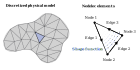
\includegraphics{figures/FEM.png}}%%
    \caption{Geometrical discretization of the physical domain into the finite element mesh, which is composed of Nedelec vector-elements. The element colored in light blue is a triangular element with three nodes and three edges, where we have sketched a quiver plot for the shape function $\mathbf{N}_2$ for Edge 2.}
    \label{fig:fem}
\end{figure}

Eigenvalue vs RHS problems


Lagrange elements vs Edge elements. Comment spurious modes.

Symmetry conditions can be applied to reduce the computational
cost of the solutions by employing perfect electric conductor (PEC) and perfect magnetic 
conductor (PMC) boundary conditions. The PEC boundary condition
imposes symmetry for magnetic fields and antisymmetry for electric fields and electric 
currents, by setting the tangential component of the electric field to zero: $\mathbf{n}\times \mathbf{E} = 0$ .
The PMC boundary condition imposes symmetry for electric fields and antisymmetry for magnetic fields
by setting the normal component of the magnetic field to zero: $\mathbf{n}\cdot \mathbf{H} = 0$.

\section{Beyond single-physics -- coupled optical systems}

Coupled multi-physics systems are physical systems where the solution of one of the physical 
problem depends on the solution of another physical problem. Let's consider that the two
problems can be described by linear partial differential equations, where the first problem
is described by the equation $\mathcal{L}_1 [\mathbf{u}]= \mathbf{a}$ and the second problem is described by the 
equation $\mathcal{L}_2 [\mathbf{w}]= \mathbf{b}$.

 If this relation is unidirectional
we call it \textbf{weak coupling}, and if the relation is bidirectional we call it 
\textbf{strong coupling}.

In weaky coupled systems, both physical problems can be solved independently in a seggregated 
manner, where the solution of one problem is used in the the other problem.

In strongly coupled systems, the physical problems are solved simultaneously.

Differentiate between weak and strong coupling.

\section{Topology optimization of multiphysics systems}

\begin{equation}
    \begin{array}{clr}
    \max\limits_{\xi} & \Phi(\xi, \mathbf{u}) & \text { (Objective function) } \\
    \text { s.t. } & \mathbf{S}_i(\xi, \mathbf{u})-\mathbf{f}_i=0 \quad \forall i \in\left[1, N_S\right] & \text { (State equations) } \\
    & c_j(\xi, \mathbf{u}) \leq 0 \quad \forall j \in\left[1, N_c\right] & \text { (Inequality constraints) } \\
    & \xi_{\text {min }} \leq \xi \leq \xi_{\text {max }} & \text { (Box constraints) }
    \end{array}
\end{equation}

The optimization problem is solved using the algorithm of the Method of Moving
Asymptotes (MMA) (CITE) and Globally Convergent Method of Moving Ssymptotes (GCMMA) (CITE).

\subsection{From densities to material properties}

To regularize the optimization and introduce a weak sense of geometric length scale, we filter
the density field using a filter operation. The filtered density can be calculated using a 
convolution-based filter operation (CITE)
\begin{equation}
    \begin{aligned}
    & \tilde{\xi}(\mathbf{r})=\frac{\sum_{k \in \mathcal{B}_{e, h}} w\left(\mathbf{r}-\mathbf{r}_k\right) A_k \xi_k}{\sum_{k \in \mathcal{B}_{e, h}} w\left(\mathbf{r}-\mathbf{r}_k\right) A_k}, \\
    & w(\mathbf{r})=\left\{r_f-|\mathbf{r}| \quad \forall|\mathbf{r}| \leq r_f, \quad r_f \geq 0, \quad \mathbf{r} \in \Omega\right.\,,
    \end{aligned}
\end{equation}

where $A_k$ is the area of the kth element, and $\mathcal{B}_{e, h}$ denotes the
$h^\text{th}$ set of finite elements whose center point is within a filter radius $r_f$ of the
$h^\text{th}$ element. One can also filter by solving a Helmholtz-type PDE (CITE):
\begin{equation}
    -\left(\frac{r_f}{2 \sqrt{3}}\right)^2 \nabla \tilde{\xi}+\tilde{\xi}=\xi
\end{equation}
The filter operation is followed by a smoothed Heaviside threshold:
\begin{equation}
    \bar{\tilde{\xi}}=\frac{\tanh (\beta \cdot \eta)+\tanh (\beta \cdot(\tilde{\xi}-\eta))}{\tanh (\beta \cdot \eta)+\tanh (\beta \cdot(1-\eta))}, \quad \beta \in[1, \infty[, \eta \in[0,1],
\end{equation}
where $\beta$ and $\eta$ control the threshold sharpness and value, respectively.

The physical field cna be interpolated to the filtered density field using a material interpolation.
In multi-physics problems, we will have one material interpolation for each different physical problem
\footnote{If the problem stem from the same physics (e.g., solving two optical problems), the material interpolation can be re-used.}.
In general, the material interpolation can be written as:
\begin{equation}
    \zeta(\bar{\tilde{\xi}})=\zeta_0+\bar{\tilde{\xi}}^p\left(\zeta_1-\zeta_0\right)
\end{equation}
where $\zeta$ is the material property, $\zeta_0$ and $\zeta_1$ are the material properties of the void and solid, respectively, and $p$
is a penalization factor (usually, $p=3$ for compliance optimization and $p$=1 for other problems). Note that for some
special cases, like optical optimization problems with metals, it is benefitial to employ a non-linear material interpolation.

Do it in such a way that it works for multiphysics.
Invert order of threshold and filter operations.

\subsection{Adjoint sensitivity analysis}

(CHECK NIELS THESIS)

The adjoint sensitivity analysis is used to efficiently calculate the gradient of the objective function with 
respect to the design variables. In this thesis, we use the adjoint sensitivity analysis  in the context of 
multi-physics problems, where multiple complex-valued PDE are solved. Let us rewrite the FOM by adding the residual
of the state equation and its complex conjugate, multiplied by the Lagrange multipliers, $\lambda_i$ and $\lambda_{i+N}$, 
respectively:
\begin{equation}
    \tilde{\Phi} =\Phi + \sum^N_i \left[ \lambda_{i}^{\top}\left(\mathbf{S}_i \mathbf{u}^*_i -\mathbf{f}_i\right) + 
    \lambda_{i+N}^{\dagger}\left(\mathbf{S}_{i}^* \mathbf{u}^*_i -\mathbf{f}_i^*\right) \right]
\end{equation}

\subsubsection*{Coupled source problems}

\subsubsection*{Coupled state-equation problems}


\section{A practical note on computational implementation}

Using first order edge, or nodal, elements a rule of thumb is to include at least 10 elements per wavelength.

Discuss direct vs iterative solvers, discuss condition number of the system.
Sparsity, symmetry, definitiness
Discuss the practical implementation, with COMSOL and other means (Fenics, gridap, etc).
Check Niels, Ian's thesis, and other references.
Bla bla bla...